\documentclass[border=10pt]{standalone}

\usepackage{tikz}
\usepackage{tikzsymbols}
\usetikzlibrary{calc,patterns,shapes.geometric}

\def\centerarc[#1](#2)(#3:#4:#5){\draw[#1] ($(#2)+({#5*cos(#3)},{#5*sin(#3)})$) arc (#3:#4:#5);}

\begin{document}
	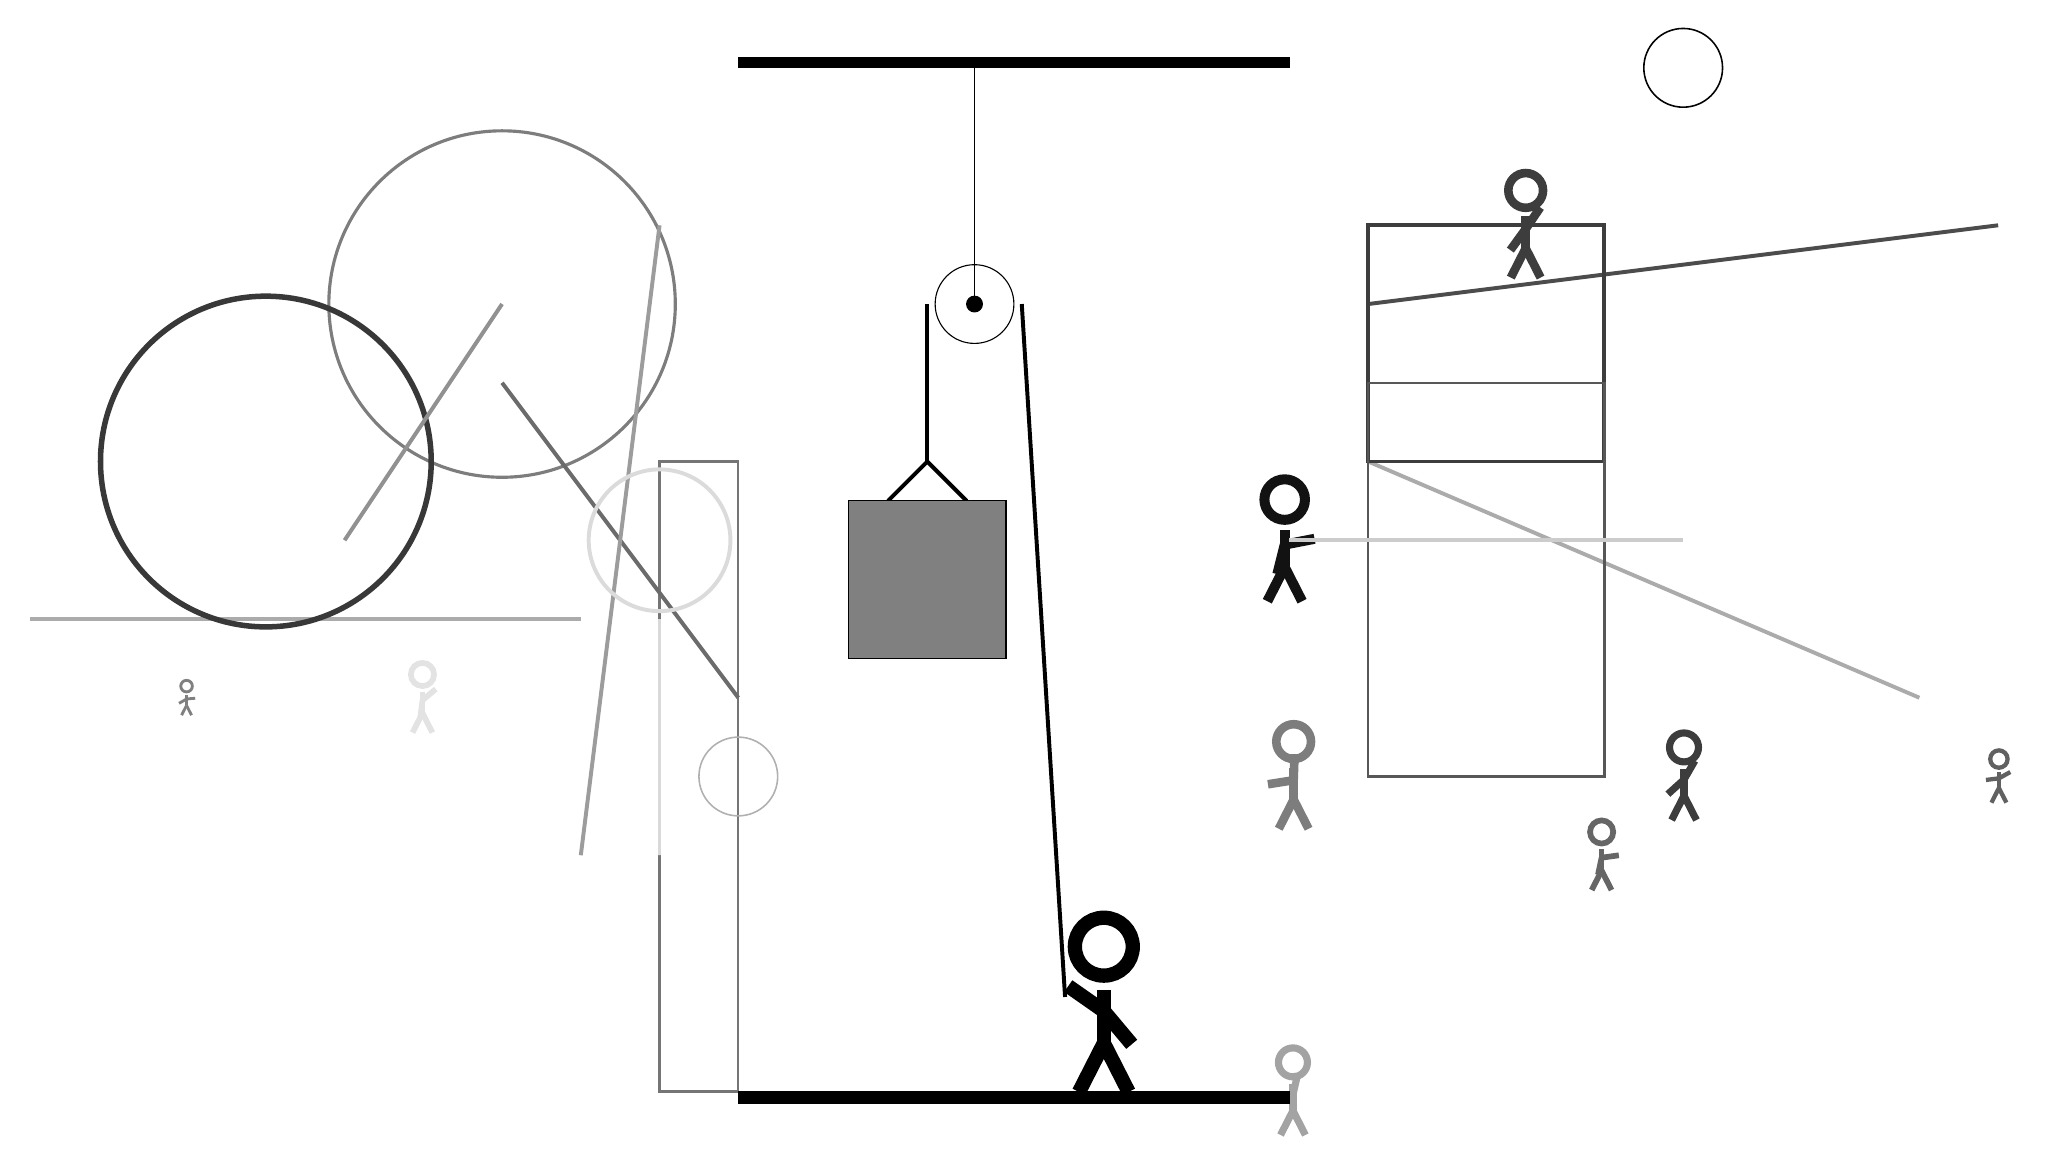
\begin{tikzpicture}
		%%%%% START %%%%%
		
		\draw[fill=black] (-2, 10) rectangle (5, 10.125);
		
		\draw (1, 7) circle (0.5);
		\draw[fill=black] (1, 7) circle (0.1);
		\draw (1, 10) -- (1, 7);
		
		\draw [line width=0.2mm, color=black!99](10, 10) circle (0.5);
		
		\draw[line width=0.5mm, color=black!33](6, 5) -- (13, 2);
		\draw[line width=0.5mm, color=black!70](6, 7) -- (14, 8);
		\node[line width=0.7mm, color=black!51] at (5, 1) {\Strichmaxerl[6][9][88]};
		\draw[line width=0.5mm, color=black!76] (6, 5) rectangle (9, 8);
		\draw [line width=0.4mm, color=black!51](-5, 7) circle (2.2);
		\draw[line width=0.3mm, color=black!54] (-3, -3) rectangle (-2, 5);
		\draw[line width=0.5mm, color=black!33](-4, 3) -- (-11, 3);
		\node[line width=0.4mm, color=black!11] at (-6, 2) {\Strichmaxerl[4][83][40]};
		
		\draw[line width=0.5mm, color=black!58](-2, 2) -- (-5, 6);
		\draw[line width=0.3mm, color=black!66] (6, 1) rectangle (9, 6);
		\node[line width=0.5mm, color=black!60] at (9, 0) {\Strichmaxerl[4][78][8]};
		\draw[line width=0.3mm, color=black!15] (-3, 0) rectangle (-3, 3);
		
		\node[line width=0.2mm, color=black!50] at (-9, 2) {\Strichmaxerl[2][30][5]};
		\node[line width=0.3mm, color=black!62] at (14, 1) {\Strichmaxerl[3][7][29]};
		\draw [line width=0.7mm, color=black!78](-8, 5) circle (2.1);
		
		\draw[line width=0.5mm, color=black!39](-3, 8) -- (-4, 0);
		
		\draw [line width=0.2mm, color=black!31](-2, 1) circle (0.5);
		\draw [line width=0.5mm, color=black!14](-3, 4) circle (0.9);
		
		\node[line width=0.5mm, color=black!36] at (5, -3) {\Strichmaxerl[5][9][77]};
		\node[line width=0.4mm, color=black!76] at (10, 1) {\Strichmaxerl[5][42][60]};
		\node[line width=0.2mm, color=black!76] at (8, 8) {\Strichmaxerl[6][54][56]};
		\draw[line width=0.5mm, color=black!43](-5, 7) -- (-7, 4);
		\node[line width=0.3mm, color=black!93] at (5, 4) {\Strichmaxerl[7][76][11]};
		\draw[line width=0.5mm, color=black!20](5, 4) -- (10, 4);
		
		
		\draw[line width=0.5mm] (-0.1, 4.5) -- (0.4, 5.0) -- (0.9, 4.5);
		\draw[fill=black!50] (-0.6, 4.5) rectangle (1.4, 2.5);
		
		\draw[line width=0.5mm] (0.4, 7) -- (0.4, 5.0);
		\centerarc[line width=0.5mm](1, 7)(0:180:0.6);
		\draw[line width=0.5mm](1.6, 7) -- (2.15, -1.8);
		
		\node at (2.6, -1.9) {\Strichmaxerl[10][-35][-50]};
		
		\draw[fill=black] (-2, -3) rectangle (5, -3.15);
		
		%%%%% END %%%%%
	\end{tikzpicture}
\end{document}